\documentclass[12pt,a4paper]{article} % this tells LaTeX to make the
\usepackage[utf8]{inputenc} 
\usepackage[boxed]{algorithm2e} 
\usepackage{cite}
\usepackage{color}
\usepackage{listings}
\usepackage{hyperref}
\lstset{ %
language=C++, % choose the language of the code
basicstyle=\footnotesize, % the size of the fonts that are used for the code
numbers=left, % where to put the line-numbers
numberstyle=\footnotesize, % the size of the fonts that are used for the line-numbers
stepnumber=0, % the step between two line-numbers. If it is 1 each line will be numbered
numbersep=5pt, % how far the line-numbers are from the code
backgroundcolor=\color{white}, % choose the background color. You must add \usepackage{color}
showspaces=false, % show spaces adding particular underscores
showstringspaces=false, % underline spaces within strings
showtabs=false, % show tabs within strings adding particular underscores
frame=single, % adds a frame around the code
tabsize=2, % sets default tabsize to 2 spaces
captionpos=b, % sets the caption-position to bottom
breaklines=true, % sets automatic line breaking
breakatwhitespace=false, % sets if automatic breaks should only happen at whitespace
escapeinside={\%}{)} % if you want to add a comment within your code
}
\usepackage{amsmath} % a very handy maths typesetting
% package from the
% American Mathematical Society
\usepackage{graphicx} % the standard
% report on a4 paper, at 12pt
% (nice and easy to read) and
% to use the report class file
% (a file that defines how the
% report should look when
% finished so that you can
% concentrate on content).
% the bit between the \documentclass statement and the
% \begin{document} statement is called the ``preamble''
% you may have noticed that comments are denoted by a % sign
\title{Group Contract - Group A3} % put in a title (if
% you want a title page
%\author{Raluca Marinescu, Eduard Paul Enoiu} % put in the author
% (if you want a title page)
\begin{document} % start of the document
\maketitle % makes the title page
\section{Members of the group}
 \begin{itemize}
\item Raluca Marinescu: \emph{rmu09001@student.mdh.se}
\item Andrea Graciela Garcia Badillo: \emph{aga09001@student.mdh.se}
\item Ivan Francisco Castro Ceron: \emph{ico09002@student.mdh.se}
\item Eduard Paul Enoiu: \emph{eeu09001@student.mdh.se} (group contact)
\end{itemize}

\section{Seminar's Topic}
 \begin{itemize}
\item \textbf{SOLVING SUDOKU WITH MATLAB}
\end{itemize}

\section{Preliminary Schedule}
\begin{center}
\begin{tabular}{ | l | l | p{8cm} |}
\hline
Meeting & Date & Agenda\\ \hline
0 & January 28 & Choosing the topic and finalizing the group contract document (\emph{done already}) \\ \hline
1 & February 1 & Different Sudoku Algorithms Analysis and GUI Development Conditions\\ \hline
2 & February 8 & Selection of Sudoku Algorithm and implementation in Matlab using command line interface and GUI  \\ \hline
3 & February 15 & Algorithm and GUI implementation evaluation and refinement \\ \hline
4 & March 1 & Implementation improvements \\ \hline
5 & March 8 & Finalizing the report and presentation \\ \hline
\end{tabular}
%\caption{Execution time for different learning tests}
\end{center}
\section{Responsibilities}
 \begin{itemize}
\item Raluca Marinescu: \textbf{Sudoku Algorithm Development}
\item Andrea Graciela Garcia Badillo: \textbf{GUI Development}
\item Ivan Francisco Castro Ceron: \textbf{GUI Development}
\item Eduard Paul Enoiu: \textbf{Sudoku Algorithm Development}
\end{itemize}
\section{Signature}
\mbox{}
\newline
\mbox{}
\newline
Raluca Marinescu \hrulefill
\mbox{}
\newline
\mbox{}
\newline
\mbox{}
\newline
\mbox{}
\newline
Andrea Graciela Garcia Badillo \hrulefill
\mbox{}
\newline
\mbox{}
\newline
\mbox{}
\newline
\mbox{}
\newline
Ivan Francisco Castro Ceron \hrulefill
\mbox{}
\newline
\mbox{}
\newline
\mbox{}
\newline
\mbox{}
\newline
Eduard Paul Enoiu  \hrulefill
\newpage

\title{February 28, 2011}
\section{Annex 1 - Group meetings activity}
\begin{center}
\begin{tabular}{ | l | l | p{8cm} |}
\hline
Meeting & Date & Agenda\\ \hline
1 & February 1 & We have divided the work. We have analyzed how to solve Sudoku puzzles. Also Andrea and Ivan began working for the GUI. They presented the first version of the GUI with no functionality. Also we have decided to work with the SVN system repository in order to have a source code versioning control: \url{https://i-sudoku-matlab.googlecode.com/svn/trunk/} \\ \hline
2 & February 8 & Raluca and Eduard Presented a first version of the algorithm for verification purposes. The algorithm was tested only in the command line version. Andrea and Ivan presented an improved version of the GUI. \\ \hline
3 & February 15 &  Andrea and Ivan improved the GUI with xls support for automatic puzzle addition. Raluca and Eduard  modified the algorithm in order to solve more complicated puzzles. We have encounter mistakes in the algorithm code and Raluca started to refine the implementation.\\ \hline
3+(Extra meeting) & February 22 & In this meeting we have refined the implementation. Ivan and Andrea added more Sudoku puzzles for testing purposes. Everything is working fine and we have started working for our Seminar 1 presentation.\\ \hline
\end{tabular}
%\caption{Execution time for different learning tests}
\end{center}

\end{document}
\section{Introduction}
Autonomous mobile robots have been extensively studied not only as an element of industrial and home automation, but also as a test bed in Robocup \cite{DBLP:conf/robocup/1997} competitions to academically establish the achievement of artificial intelligence. One of the essential and critical research areas in autonomous robotics is the learning ability which supports robots to autonomously navigate and adapt to a given environment without human guidance. Reinforcement Learning (RL) is a machine learning technique that defines a certain scenario, where a robot attempts to improve its behaviour by taking actions and receiving rewards or punishments. Because RL enables an $agent$\footnote{We will use in this report the term $agent$ when refering to the robot's model used in RL algorithm} to learn autonomously from its own environment and experience, it is a well suited framework for learning control policies for mobile robots.
\newline
\\ One of the problems of using this kind of technique is that it requires a long period of training for learning an acceptable policy and it is considered very slow for robot implementations as we have shown previously in \cite{enoiusoccer}. In order to solve or at least to reduce this problem, we show here an implementation of a parallel model of RL suitable for multi-core configurations of processors. One of the well known RL algorithms is Q-learning which we have chosen by means of simplicity.
\newline
\\ This report is organized as follows: Section 2 presents some theoretical background and the formal model used normally for RL. Section 3, overviews the Q-learning algorithm in his sequential form. Section 4 shows general issues and details about the parallel model that we want to implement. In section 5 we show a particular experiment and some results, concluding the paper in section 6.
\section{Background}
RL is a machine learning paradigm that offers algorithms for optimizing an agent's behaviour by using the capability of the agent to sense rewards from the environment. An agent in our approach can be considered a robot that interacts with the environment by its sensors and actuators (motors).
Let us assume that the agent, whose behaviour is described by the RL paradigm, is working in discrete time steps. We denote by $S$ the finite discrete set of states, and by $A$ the set of actions. In each time step $t$, the agent determines its actual state and executes one action. Therefore, agent's life phase (as depicted in Figure 1) can be written as a finite sequence $t_{0} a_{0} r_{0} t_{1} a_{1} r_{1} ... t_{n} a_{n} r_{n} $, where $t_{n}$ indicates how many times an agent makes observations using the sensors, $a_{n}\in $ A represents an action, and $r_{n}\in $ R represents an reward, that was received at time $n$.
\begin{figure}
\begin{center} 
\includegraphics[width=0.50\textwidth]{standard.png} 
\caption{Standard Model of RL.}
\end{center} 
\end{figure}
\newline
\\ In autonomous robot navigation, each state $s$ is a location (cell) in the grid-based environment and each observation is a discrete perception that can be produced by the robot sensors. If the objective of the robot is to reach a particular goal state, then the reward will be maximized when the robot has reached this particular state.
\newline
\\ Next we assume that the robot does not need a history of previous observations to make decisions. In \cite{sutton1998reinforcement} this assumption is called the Markov property. The decision is centred on the last observation $t_{n}$ only. The agent's task is to find a policy $\pi$, which decides what action should be chosen in a specific state. Let us accept also that the policy can be defined as function $\pi : S \rightarrow A$, where $\pi(s_{n}) = a_{n}$. For optimal reasons, the task is to find a strategy $\pi^{*}$ that get the most out of the expected cumulative reward $V^{\pi^{*}}(s_{n})$. The expected reward, if the agent starts in state $s_{t}$ and follows policy $\pi$, is 
\begin{equation}V^{\pi^{*}}(s_{n}) =r_{n} + \gamma r_{n+1} + \gamma^{2} r_{n+2}+ \cdots = \sum_{i=0} \gamma^{i} r_{n+1}. \end{equation}
In equation (1), $0 \leq \gamma \leq 1$ is a constant which defines the value of delayed versus immediate rewards.
\\ In the next section we will describe Q-learning, one of the most used RL algorithms in Machine Learning.
\section{Q-learning}
Q-learning algorithm was the first algorithm to compute optimal strategy $\pi^{*}$ \cite{watkins1992q}. The basic notion behind the algorithm is to define the $Q$-values. $Q^{\pi}(s,a)$ is the expected reward if the agent takes action $a$ in state $s$ and follows policy $\pi$:
\begin{equation} Q^{\pi}(s,a) = r(s,a) + \gamma V^{\pi}(s^{'}), \end{equation}
where $s^{'}$ is the state, in which the agent is by taking action $a$ in state $s$.
\begin{algorithm}
\KwIn{$S$, $A$ and $Q(s,a)$}
\KwOut{$Q(s,a)$}
Observe current state $s$\;
\Repeat{terminal state is reached}{
Choose and execute action $a$\;
Observe reward $r$\;
Observe new state $s^{'}$\;
$Q(s,a) \leftarrow r + \gamma \max_{a^{'}} Q(s^{'}, a^{'})$\;
$s \leftarrow s^{'}$\;
}
\caption{Q-learning algorithm}
\end{algorithm}
\newline
\\ Q-learning algorithm is shown in Algorithm 1. It guarantees convergence to optimal values of $Q^{\pi}(s,a)$, if $Q$-values are represented without any function approximations, rewards are bounded and every state-action pair is visited infinitely often. 
\\ In practice the learning task is split in episodes where each episode starts in a initial state and ends in a goal state.
\section{Parallel Q-learning}
One of the problems of Q-learning algorithm is that the agent requires a great number of training episodes to learn an acceptable value as we have shown in \cite{enoiusoccer}. There are three principal approaches for speeding up the learning process:
\begin{enumerate}
\item using multiple input of information from external observers \cite{maclin1996creating},
\item using learning and planning combined \cite{lin1992self} \cite{moore1993prioritized} and
\item using a parallel implementation of the Q-learning algorithm \cite{printista2002parallel}.
\end{enumerate}
We will use the third alternative, which is based upon a parallel implementation of the Q-learning algorithms. The tasks will be distributed among processors in a parallel way. The main motivation goal is to increase the processing speed. The parallel implementation is based usually on some partitioning strategy which divides the problem in different parts. We use training decomposition by dividing the training episodes in different fractions. To model in simple way the environment’s states we use the classic tabular approach as depicted in Figure 2. The robot is depicted in the middle with eight possible actions and the states are depicted from A to Z.
\begin{figure}
\begin{center} 
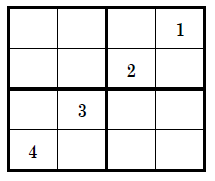
\includegraphics[width=0.55\textwidth]{1.png} 
\caption{Agent's possible movements}
\end{center} 
\end{figure}
\newline
By using this model and the episodic training paradigm, a partitioning technique can be applied to the function of the algorithm. Therefore, in order to divide the original sequential program in parallel independent units implies to identify relations between different modules where parallel implementation can be applied. We have divided the training episodes in a way that each thread will be focused only on a subgroup of all training episodes.
\section{Experimental results}
This section presents a comprehensive analysis of the results by testing the sequential approach of Q learning and our parallel implementation. 
\subsection{Experiment description}
For an accurate comparison we have used a two dimensional grid similar to the experiments used in \cite{enoiusoccer}. For our case, we have used a grid of $16 X 12$ cells. In each cell the agent has eight possible actions: RIGHT, LEFT, DOWN, UP and all four diagonals. By choosing one of the actions the agent deterministically moves to the corresponding neighbour cell. When the agent reaches the goal it receives 100 units. Each non-terminal transition produces a reward of 0 units from the environment and when it reaches an obstacle it receives a negative reward of -100 units. The discount factor $\gamma$ is 0.8. We start every episode in a random state in the environment. This process is repeated after finalizing every training episode. In our experiment the end of the episode is determined when the agent reaches the goal state. 
\newline
\\ For implementing this parallel approach to Q-learning we have used two of the most used shared-memory parallel programming models: OpenMP and Pthreads. All the source code was written in C using OpenMP API and Pthreads libraries. The system used for testing our implementations was an AMILO Pro Notebook with Intel Core 2 CPU with 1.66 Ghz and Mandriva Linux as operating system.
\newline
\\ Also for compiling all three implementations ($ql-serial.c$ , $ql-paralel1.c$ and $ql-paralel2.c$) it is necessary to use the next shell commands:
\begin{lstlisting}
gcc -o ql-serial ql-serial.c
gcc -fopenmp -o ql-paralel1 ql-paralel1.c
gcc -pthread -o ql-paralel2 ql-paralel2.c
\end{lstlisting}
\subsection{Sequential Q-learning implementation}
The sequential implementation is following the algorithm described in section 3. First we have defined the positions on the field for every state from 0 to 191 as depicted next:
\begin{lstlisting}
for (i=0; i<h; i++)
for (j=0; j<w; j++)
{
field[i][j]=count1;
count1=count1+1;
}
\end{lstlisting}
The Q and R matrices are populated with 0 (start of learning) and -100 (no transition is possible) respectively: 
\begin{lstlisting}
for (i=0; i<h*w; i++)
for (j=0; j<h*w; j++)
{
q[i][j]=0.0;
}
for (i=0; i<h*w; i++)
for (j=0; j<h*w; j++)
{
r[i][j]=-100;
}
\end{lstlisting}
After defining the Q and R matrices we introduce all the eight possible transitions to the neighbour states in the R matrix:
\begin{lstlisting}
for (i=0; i<h; i++)
for (j=0; j<w; j++)
{
if (i>0)
r[field[i][j]][field[i-1][j]]=0;
if (j>0)
r[field[i][j]][field[i][j-1]]=0;
if (i<(h-1))
r[field[i][j]][field[i+1][j]]=0;
if (j<(w-1))
r[field[i][j]][field[i][j+1]]=0;
if ((i>0)&&(j>0))
r[field[i][j]][field[i-1][j-1]]=0;
if ((i>0)&&(j<(w-1)))
r[field[i][j]][field[i-1][j+1]]=0;
if ((i<(h-1))&&(j>0))
r[field[i][j]][field[i+1][j-1]]=0;
if ((i<(h-1))&&(j<(w-1)))
r[field[i][j]][field[i+1][j+1]]=0;
} 
\end{lstlisting}
Also we are marking the goal state and introduce the reward for the goal state in the R matrix as depicted below:
\begin{lstlisting}
r[field[c1goal][c2goal]][field[c1goal][c2goal]]=100;
if (c1goal>0) 
r[field[c1goal-1][c2goal]][field[c1goal][c2goal]]=100;
if (c2goal>0)
r[field[c1goal][c2goal-1]][field[c1goal][c2goal]]=100;
if (c1goal<(h-1)) 
r[field[c1goal+1][c2goal]][field[c1goal][c2goal]]=100;
if (c2goal<(w-1))
r[field[c1goal][c2goal+1]][field[c1goal][c2goal]]=100;
if ((c1goal>0)&&(c2goal>0))
r[field[c1goal-1][c2goal-1]][field[c1goal][c2goal]]=100;
if ((c1goal>0)&&(c2goal<(w-1)))
r[field[c1goal-1][c2goal+1]][field[c1goal][c2goal]]=100;
if ((c1goal<(h-1))&&(c2goal>0))
r[field[c1goal+1][c2goal-1]][field[c1goal][c2goal]]=100;
if ((c1goal<(h-1))&&(c2goal<(w-1)))
r[field[c1goal+1][c2goal+1]][field[c1goal][c2goal]]=100;
\end{lstlisting}
The learning algorithm has 10000 learning episodes. Every episode starts in a random position: 
\begin{lstlisting}
start=randint(h*w);
pos=start;
flag=0;
\end{lstlisting}
The $flag$ variable is used for signalling when the agent has reached the goal state. As long as $flag =0$ the agent is not in the goal state and it should check the possible movements it can do:
\begin{lstlisting}
for(j=0; j<h*w; j++)
{
if (r[pos][j]>-100)
{
pos_mov[count4]=j;
count4=count4+1;
}
}
\end{lstlisting}
After checking the possible movements the agent should choose, accordingly with the algorithm, a new random movement: 
\begin{lstlisting}
new_pos=pos_mov[randint(count4)];
\end{lstlisting}
At every step of the learning we update the Q matrix with the values given by the Q-learning algorithm:
\begin{lstlisting}
for(j=0; j<h*w; j++)
{
if (q[new_pos][j]>max) max=q[new_pos][j];
}
q[pos][new_pos]=(float)r[pos][new_pos]+v*max;
\end{lstlisting}
At the end of the learning process we can put the agent to navigate in the environment without hitting any objects. We have observed that the training can be decomposed and will address this in the next sections. We have parallelized only the learning algorithm and not the Q and R values definition because our goal was to evaluate the performance strictly for the learning part of the program.
\subsection{OpenMP implementation of Q-learning}
For the OpenMP implementation we've used the start position, current position, flag and other variables as private for every thread except the $Q$ matrix and the $count2$ variable that are shared between threads:
\begin{lstlisting}
#pragma omp parallel for private(start, pos, flag, pos_mov, count4, new_pos, max, i, j) shared(count2,q)
\end{lstlisting}
By using this directive of parallelization every thread is writing concurrently in the Q matrix. Therefore, all threads are doing concurrently the training episodes until the $count2$ variable equals 10000 and the training halts. Because of the large number of iterations and the random character of the algorithm we didn’t used any writing protection on the Q matrix.
\subsection{Pthreads implementation of Q-learning}
In the case of using Pthreads we've begun with separating the main function for parallel execution. As in OpenMP implementation all the variables needed for the training episode are private. We have divided the total number of episodes by the number of threads used as shown below (where P is the number of processors and N is the number of episodes): 
\begin{lstlisting}
for(count2=id*(N/P); count2<(id+1)*(N/P); count2++)
\end{lstlisting}
The body of the thread contains the learning algorithm done in every episode including the random position definition, the possible movements and the updates for Q values. Every thread is doing the designated number of episodes concurrently until the count variable is equal with 10000. The threads creation and the learning process's start are done in the same way as shown below:
\begin{lstlisting}
for (i = 0; i < P; ++i)
{
pthread_create(&thread[i], &attr, body, (void*)i);
}
pthread_attr_destroy(&attr);
for (i = 0; i < P; ++i)
{
pthread_join(thread[i], NULL);
}
\end{lstlisting}
As in the OpenMP case, because of the large number of iterations and the random character of the algorithm we didn’t used any writing protection on the Q matrix.
\subsection{Results}
The parallel Q-learning version was executed on a system with 2 processors\footnote{The code was tested with the system described in section 5.1}. The whole set of episodes was divided among current cores. In Table 1 we show the execution times for the parallel and sequential algorithms where they converged to the optimal policy. The execution times are in seconds and correspond to five different results.
\begin{table}
\begin{center}
\begin{tabular}{ | l | l | p{2cm} |}
\hline
Sequential & OpenMP & Pthreads\\ \hline
11.604053 & 6.830415 & 6.880469 \\ \hline
11.813076 & 6.776290 & 7.124108 \\ \hline
11.852998 & 7.327573 & 7.163377 \\ \hline
11.530325 & 7.130383 & 7.106525 \\ \hline
11.700858 & 7.133425 & 7.135284 \\ \hline
\end{tabular}
\caption{Execution time for different learning tests}
\end{center}
\end{table}
\newline
\\ Table 2 shows the parallel version’s performance. The parallel algorithm shows a speedup of 1.6 over the sequential one. This indicates that an increment in the number of processors can improve its time but the policy will not be improved because the number of training episodes is limited by definition.
\begin{table}
\begin{center}
\begin{tabular}{ | l | l | p{2cm} |}
\hline
Algorithm & Average Execution Time & Speedup\\ \hline
Sequential & 11.698 & - \\ \hline
OpenMP & 7.046 & 1.660 \\ \hline
Pthreads & 7.078 & 1.652 \\ \hline
\end{tabular}
\caption{Achieved speed-ups for the two parallel implementations}
\end{center}
\end{table}
The learned policy is comparable for every tested implementation and as a result we can infer that the agent is following the same path in every test implementation and therefore the policy performance is similar in all test cases.
\section{Conclusions}
In this report, we have presented a parallel implementation of the Q-learning algorithm based on training episodes partitioning. The results show the feasibility of the approach related to the speedup even for small grid with 192 states. We can say that the current results will benefit a real obstacle avoidance problem with thousand or million states. We have shown also that functional decomposition for the training episodes is easy to scale to larger problems.
\newline
\\Also work should be done in the future to extend this approach by means of using other reinforcement learning algorithms like SARSA that are more suitable to dynamic environments.
%\bibliography{mybib}{}
%\bibliographystyle{plain}


